\section{Demonstration}
Our demo system is implemented in .NET environment on a workstation with
3.2 GHz Dual-core i5 and 14GB RAM.
A snapshot of our system is shown in \figref{fig:sysdemo}. Our system provides
 several variants of context extraction and clustering algorithms
for comparison purposes.
 \tabref{tab:op} shows the configurable options for users.
If the user choose TSC as clustering method, the Representation option is
fixed to Conceptualization, and the Context options is fixed to Sibling.
 Our system can provide 19 kinds of combination of methods for comparison.

\begin{figure}[th]
\begin{center}
\centering
\includegraphics[width=80mm]{sysdemo.eps}
\caption{System snapshot}
\label{fig:sysdemo}
\end{center}
\end{figure}

\begin{table}[th]
\centering \small
\caption{Various configurations of the demo system}
\begin{tabular}{|l|l|l|}
\hline
{\bf Context} & {\bf Representation} & {\bf Clustering} \\
\hline
      Whole &        BOW &         AP \\

   Sibling &        Conceptualization &        HAC \\

Sibling(Image only) &        BOC &           TSC \\
\hline
\end{tabular}
\label{tab:op}
\end{table}

For the context extraction process, we provide options such as {\em Whole},
{\em Sibling}, and {\em Sibling(Image only)}.
The \textit{Whole} option uses the text of the whole page as context.
\textit{Sibling} consider both of the image context and query string context,
which is proposed in our system.
\textit{Sibling (Image only)} provides an option of only using the text
around the image as context.

Similar to context extraction, there are three context representations \textit{BOW, Conceptualization, BOC} in the system.
BOC stands for "bag-of-concepts", in which we detect Wikipedia terms without explicitly
disambiguate the sense of the terms.
User can also select the clustering method such as
TSC, \textit{Affinity Propagation(AP)}\cite{Frey07ap} and HAC, and tune the threshold for each clustering method.

We offer 56 query strings for testing.
These queries were downloaded in advance since the
Google Image search engine is not always available in
our part of the world. Besides the 56 pre-loaded queries,
user can enter new queries in the search box. But the download process
may take a long time. The \textit{Top} option
indicates that we are processing the top $K$ images
retrieved from search engine.

\figref{fig:kiwi-cluster} shows two largest clusters of ``kiwi'' from a total
of 100 images.
The accuracy (purity, F1, NMI) of the result are shown on the top,
and the clusters are listed below.
In this particular result, only one kiwi bird image is incorrectly
grouped into the kiwifruit cluster since its text is more about kiwifruit
than about kiwi bird.
%It is an exception, whose context does not closely describe the image.
%Since it is not very common, we can ignore this kind of exceptions.

\begin{figure}[th]
\begin{minipage}[t]{0.5\linewidth}
\centering
\includegraphics[width=0.98\columnwidth]{kiwi_fruit.eps}
%\caption{Cluster of fruit kiwi}
%\label{fig:side:a}
\end{minipage}%
\begin{minipage}[t]{0.5\linewidth}
\centering
\includegraphics[width=0.98\columnwidth]{kiwi_bird.eps}
\end{minipage}
\caption{Two clusters of kiwi}
\label{fig:kiwi-cluster}
\end{figure}

In our system, for each cluster, we list the top 10 most
representative concepts to describe each cluster.
For example, the left sub-figure of \figref{fig:kiwi-cluster}
shows a cluster about
\textit{Kiwifruit, Fruit}, etc. while the right sub-figure shows a cluster
about \textit{Bird, Kiwi}, etc. (Notice that ``Kiwi'' is the term for
kiwi the bird in Wikipedia.)

The demo system also keeps track of the context extraction process.
When the user clicks on an image in the result set,
the system will open the original web page in the browser.
If the user clicks on the \textit{context} link,
the system will show the contexts (both tag and text context).
At the end of the context page, there is a ranked list of
Wikipedia concepts extracted from the context. \figref{fig:kiwi-context} shows
the original web page (top) and the context (bottom) of an image of kiwifruit.

\begin{figure}[th]
%\begin{minipage}[t]{\columnwidth}
\centering
\includegraphics[width=\columnwidth]{kiwi_ori.eps}
\\
\vspace*{4pt}
%\label{fig:side:a}
%\end{minipage}%
%\begin{minipage}[t]{\columnwidth}
%\centering
\includegraphics[width=\columnwidth]{kiwi_ctx.eps}
%\end{minipage}
\caption{Context extraction}
\label{fig:kiwi-context}
\end{figure}
